\documentclass[a4paper,12pt,notitlepage,oneside]{article}

\usepackage[utf8]{inputenc}
\usepackage[greek,english,french]{babel}
\usepackage[cyr]{aeguill}
\usepackage{enumitem}
\usepackage{float}
\AtBeginDocument{
   \renewcommand\tablename{\textsc{Tableau}}
   \renewcommand\figurename{\textsc{Figure}}
}
\usepackage{graphicx}          
\usepackage{tabularx} 
\usepackage{multirow}   
\usepackage{color}
\definecolor{ENSblue}{RGB}{0,119,139}
\usepackage[backref=true,colorlinks=true,linkcolor=ENSblue,urlcolor=ENSblue]{hyperref}
\addtolength{\textwidth}{4cm}
\addtolength{\oddsidemargin}{-2cm}
\addtolength{\topmargin}{-1.8cm}
\addtolength{\textheight}{3.6cm}
\usepackage{verbatim}
\usepackage{amsmath}
\usepackage{fancyhdr}
\usepackage{titlesec}
\usepackage{amsmath,amssymb}
%%%%%%%%%%%%%%%%%%%%%%%%%%%%%%%%%%%%%%%%%%%%%%%%%%%%%%%%%%%%%%%%%%%%%%%%%%%%%%

\author{Dubresson Matteo} 
\title{TP2 \\ Utilisation du langage assembleur sur ARM Cortex M0+}
\date{}
\pagestyle{plain}
\begin{document}
\pagestyle{fancy}
\fancyhf{}
\fancyhead[L]{TP2 441} % à gauche
\fancyhead[R]{Matteo DUBRESSON} % à droite
\fancyfoot[C]{\thepage} % numéro de page centré
\maketitle
\vspace{1 cm}
\begin{center}
--  \today~ --
\end{center}
\vspace{1 cm}




\begin{figure}[H]
    \centering
    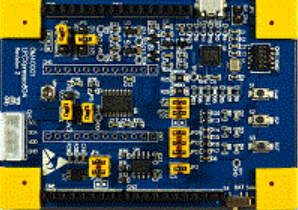
\includegraphics[width=0.5\linewidth]{2026-09-26-20-42-44.png}
    \caption{LPC804 utilisé}
    \label{fig:${imageFileNameWithoutExt}}
\end{figure}


\tableofcontents

\maketitle

\bigskip

\newpage

\section{Préparation}

\subsection*{P.1}

Dans la documentation du LPC804, on peut retrouver les adresses de ces différents registres. 

\[ \text{SYSAHBCLKCTRL0 :} ~~0x4004~8080 ~~|~~ 0100~0000~0000~0000~0100~1000~0000~1000~0000\]

\[ \text{DIR0 :} ~~0xA000~2000 ~~|~~ 1010~0000~0000~0000~0010~0000~0000~0000\]

\subsection*{P.2}

Dans la documentation des processeurs ARMv6-M, on retrouve page A1-26 que les instructions sont codées sur 32 bits. 

\subsection*{P.3}

La ligne 10 du code active l'horloge des périphériques GPIO et IOCON. On réalise un |= pour ne pas changer les périphériques déjà activés. On combine également les deux périphériques avec un | pour pouvoir réaliser l'opération en une seule fois.

\subsection*{P.4}

Dans le code assembleur présenté, on retrouve plusieurs instructions : 

\begin{itemize}
   \item movs r3,\#x : permet de mettre une valeur x dans un registre r3.
   \item lsls r2,r3,\#y : permet de décaler les bits du registre r3 vers la gauche de y positions et la stocker dans r2.
   \item ldr r1,[r0,r2] : permet de lire la valeur à l'adresse contenue dans r0 + r2 et de la stocker dans r1.
   \item orrs r1,r3 : fait r1 |= r3.
   \item str r1,[r0,r2] : permet d'écrire la valeur contenue dans r1 à l'adresse contenue dans r0 + r2.
\end{itemize}

\subsection*{P.5}

\noindent Le \# sert à désigner une valeur immédiate et non un registre. 
\\
\\
Le [~] sert à désigner une adresse mémoire.

\subsection*{P.6}

On commence par mettre $0xA0$ dans $R3$, on le décale de 24 bits puis on le met dans $R2$. \\
On réalise la même opération avec $0x80$ mais on le décale de 6 bits. \\
En sommant les deux dans $R3$, on obtient $0xA000~2000$ qui est l'adresse du registre DIR0. \\

On peut donc récupérer la valeur du registre DIR0, la suite du code servant à d'autres opérations. 



\section{Manipulation 1}

\subsection*{1.1}

Parmis les différents registres utilisés : 

\begin{itemize}
   \item SYSAHBCLKCTRL0 : permet d'activer l'horloge des périphériques GPIO et IOCON.
   \item DIR0 : permet de configurer les broches du port 0 en entrée ou en sortie.
   \item GPIO\_PORT\_NOT0 : permet d'inverser l'état du port 0.
\end{itemize}


\subsection*{1.2}

Lorsqu'on implémente le code dans le microcontrôleur, on peut observer que la LED s'allume et s'éteint à une période de 0,57 s

\subsection*{1.3}

Lorsqu'on lance le code dans l'onglet désassembleur, on constate que 48 instructions sont nécessaires pour exécuter la fonction main. 

\vspace{1cm}

\section{Manipulation 2}

\subsection*{2.1}

Les directives qui ne génèrent pas de code sont :
\begin{itemize}
   \item .syntax
   \item .equ
   \item boucle / bne boucle
\end{itemize}

Tandis que les instructions qui génèrent du code sont :

\begin{itemize}
   \item ldr
   \item str
   \item subs
\end{itemize}

\subsection*{2.2}

Les instructions ont pour tache 

\begin{itemize}
   \item ldr R,\#x : permet de charger la valeur x dans le registre R.
   \item str R1,[R2,\#0] : permet d'écrire la valeur contenue dans R1 à l'adresse contenue dans R2.
   \item subs R6,\#1 : fait R6-=1
\end{itemize}

On peut réécrire l'algorithme sous forme de pseudo-code :


\begin{center}
\begin{minipage}{0.6\textwidth} % Ajuste la largeur (ici 60% de la largeur de page)
\begin{tabbing}
\hspace{1cm} \= \hspace{1cm} \= \kill 
tant que \\
\> GPIO\_PORT\_NOT0 = 0xa0002300 \\
\> LED4 = $(1 \ll 11)$ \\
\> init\_cpt = 2000 \\
\> stocker LED4 à l'adresse GPIO\_PORT\_NOT0 \\
\> tant que init\_cpt non nul  \\
\> \> init\_cpt $-=$ 1
\end{tabbing}
\end{minipage}
\end{center}

\subsection*{2.3}

Lors de l'exécution des instructions 0x334 à 0x338, on fait : 

\begin {enumerate} [start = 334] 
   \item ldr r6 [pc,\#20] @0x34c $<boucle+22>$ : on charge dans r6 la valeur contenue à l'adresse pc+20, soit 0x34c. On obtient donc r6 = 2000.
   \addtocounter{enumi}{1}
   \item subs r6,\#1 : on décrémente r6 de 1 
   \addtocounter{enumi}{1}
   \item bne.n 0x336 $<main+54>$ : on teste si r6 est nul, si ce n'est pas le cas on retourne à l'adresse 0x336.
\end{enumerate}

\subsection*{2.4}

Maintenant qu'on a optimisé le code, on peut observer que la LED s'allume et s'éteint avec une période beaucoup plus courte, d'environ 0,15 s (compliquer à mesurer précisément car clignote très vite). 

\subsection*{2.5}

Si on analyse l'implémentation des instructions ldr, on peut constater que 

\subsection*{2.6}

Dans la documentation, on comprend que le s sert à faire une mise à jour du drapeau de condition. 

\subsection*{2.7}

Bne signifie \textit{branch if not equal}, ainsi dans une instruction du type bne boucle : 

\begin{itemize}
   \item si le drapeau Z == 0 : on continue la boucle
   \item si le drapeau Z == 1 : on sort de la boucle
\end{itemize}


\vspace{1cm}


\section{Manipulation 3}

\subsection*{3.1}

On a intégré la boucle infinie au code assembleur dans la fonction main2.
En faisant ça le code rédigé à la main est beaucoup plus optimisé : la boucle d'attente ne fais plus que deux instructions (subs, bne), ce qui veut dire qu'elle s'exécutera plus vite qu'en C, donc on aura un gain de temps significatif. 

\subsection*{3.2}

Dans le programme en C on déclare le main2() à la ligne 14, et comme dans le code assembleur on fait un global .main2, on rend visible la fonction pour assurer sa liaison entre les différents fichiers. 

\subsection*{3.3 / 3.4}

Comme le code qu'on rajoute dans le fichier assembleur correspond à l'initialisation de la tache qu'on fait, et non les consignes qu'on effectue en boucle, le gain de temps sera non significatif. 

\subsection*{3.5}

Le programme en C prend une quinzaine de lignes à écrire, et est moins complexe pour un utilisateur à faire. 
Le programme assembleur prend 20 lignes de plus à écrire, et est moins évident à écrire car on doit détailler toutes les opérations et faire bien attention aux registres qu'on utilise à chaque fois. 

\subsection*{3.6}

Cependant, malgré les réponses données en 3.5, étant donné qu'on peut agir directement sur les consignes qu'on demande, on peut simplifier grandement le temps de calcul. Le code assembleur a donc cette utilité : éviter de se reposer sur des instructions pré-construites par le langage C qui ne sont pas optimisées dans tout les cas de figure. 

\end{document}
